% Standalone TikZ figure (compile to PDF/SVG for embedding in Markdown).
\documentclass[tikz,border=2pt]{standalone}
\usepackage{tikz}
\usepackage{xcolor}
\usetikzlibrary{arrows.meta,positioning,matrix}

\begin{document}
\pagecolor{white}\color{black}
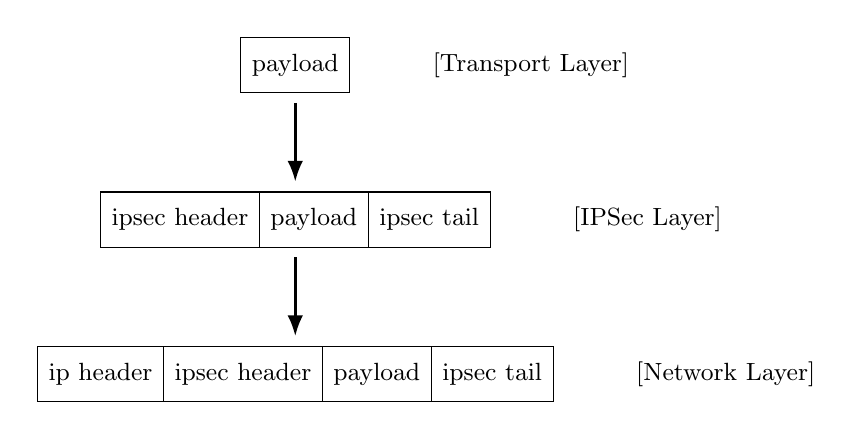
\begin{tikzpicture}[
  token/.style={draw, rectangle, minimum height=7mm, inner xsep=4pt, inner ysep=2pt, outer sep=0pt, font=\small},
  label/.style={font=\small, text=black},
  flow/.style={-Latex, line width=1pt, draw=black},
  % column sep is slightly negative so adjacent borders visually merge.
  row/.style={matrix of nodes, nodes={token}, row sep=0pt, column sep=-0.4pt},
]

% Transport layer
\matrix[row] (t0) {
  payload \\
};
\node[label, right=8mm of t0.east] (t0lbl) {[Transport Layer]};

% IPSec layer
\matrix[row, below=10mm of t0] (t1) {
  ipsec header & payload & ipsec tail \\
};
\node[label, right=8mm of t1.east] (t1lbl) {[IPSec Layer]};

% Network layer
\matrix[row, below=10mm of t1] (t2) {
  ip header & ipsec header & payload & ipsec tail \\
};
\node[label, right=8mm of t2.east] (t2lbl) {[Network Layer]};

\draw[flow] (t0.south) -- (t1.north);
\draw[flow] (t1.south) -- (t2.north);

\end{tikzpicture}
\end{document}
